\documentclass[a4paper,12pt]{article}

% --- Подключение пакетов ---
\usepackage[T2A]{fontenc}
\usepackage[utf8]{inputenc}
\usepackage[russian]{babel}

\usepackage{amsmath}
\usepackage{amssymb}
\usepackage{amsfonts} % Мат. символы

\usepackage{graphicx} % Для вставки картинок
\usepackage{geometry} % Поля страницы
\usepackage{listings} % Для вставки кода
\usepackage{xcolor}   % Цвета для кода
\usepackage{hyperref} % Гиперссылки
\usepackage{float}    % Плавающие объекты

% --- Настройка полей ---
\geometry{left=2cm, right=1.5cm, top=2cm, bottom=2cm}

% --- Авторская настройка для адекватной вставки кода с использованием кириллицы ---
\lstdefinestyle{mypython}{
    language=Python,
    basicstyle=\ttfamily\scriptsize,
    keywordstyle=\color{blue}\bfseries,
    stringstyle=\color{red},
    commentstyle=\color{green!60!black},
    numbers=left,
    numberstyle=\tiny\color{gray},
    stepnumber=1,
    numbersep=8pt,
    showspaces=false,
    showstringspaces=false,
    tabsize=4,
    frame=single,
    rulecolor=\color{black},
    breaklines=true,
    breakatwhitespace=false,
    captionpos=b,
    xleftmargin=15pt,
    xrightmargin=5pt,
    framexleftmargin=12pt,
    backgroundcolor=\color{gray!5},
    literate=%
        {а}{{\cyra}}1 {б}{{\cyrb}}1 {в}{{\cyrv}}1 {г}{{\cyrg}}1 {д}{{\cyrd}}1
        {е}{{\cyre}}1 {ё}{{\cyrie}}1 {ж}{{\cyrzh}}1 {з}{{\cyrz}}1 {и}{{\cyri}}1
        {й}{{\cyrishrt}}1 {к}{{\cyrk}}1 {л}{{\cyrl}}1 {м}{{\cyrm}}1 {н}{{\cyrn}}1
        {о}{{\cyro}}1 {п}{{\cyrp}}1 {р}{{\cyrr}}1 {с}{{\cyrs}}1 {т}{{\cyrt}}1
        {у}{{\cyru}}1 {ф}{{\cyrf}}1 {х}{{\cyrh}}1 {ц}{{\cyrc}}1 {ч}{{\cyrch}}1
        {ш}{{\cyrsh}}1 {щ}{{\cyrshch}}1 {ъ}{{\cyrhrdsn}}1 {ы}{{\cyrery}}1
        {ь}{{\cyrsftsn}}1 {э}{{\cyrerev}}1 {ю}{{\cyryu}}1 {я}{{\cyrya}}1
        {А}{{\CYRA}}1 {Б}{{\CYRB}}1 {В}{{\CYRV}}1 {Г}{{\CYRG}}1 {Д}{{\CYRD}}1
        {Е}{{\CYRE}}1 {Ё}{{\CYRIE}}1 {Ж}{{\CYRZH}}1 {З}{{\CYRZ}}1 {И}{{\CYRI}}1
        {Й}{{\CYRISHRT}}1 {К}{{\CYRK}}1 {Л}{{\CYRL}}1 {М}{{\CYRM}}1 {Н}{{\CYRN}}1
        {О}{{\CYRO}}1 {П}{{\CYRP}}1 {Р}{{\CYRR}}1 {С}{{\CYRS}}1 {Т}{{\CYRT}}1
        {У}{{\CYRU}}1 {Ф}{{\CYRF}}1 {Х}{{\CYRH}}1 {Ц}{{\CYRC}}1 {Ч}{{\CYRCH}}1
        {Ш}{{\CYRSH}}1 {Щ}{{\CYRSHCH}}1 {Ъ}{{\CYRHRDSN}}1 {Ы}{{\CYRERY}}1
        {Ь}{{\CYRSFTSN}}1 {Э}{{\CYREREV}}1 {Ю}{{\CYRYU}}1 {Я}{{\CYRYA}}1
}
\lstset{style=mypython}

\begin{document}

% ===========================================================================
% 1. ТИТУЛЬНЫЙ ЛИСТ
% ===========================================================================
\begin{titlepage}
    \centering
    % Шапка
    {\fontsize{11}{13}\selectfont \textbf{Министерство науки и высшего образования Российской Федерации}} \\
    {\fontsize{7}{10}\selectfont ФЕДЕРАЛЬНОЕ ГОСУДАРСТВЕННОЕ АВТОНОМНОЕ ОБРАЗОВАТЕЛЬНОЕ УЧРЕЖДЕНИЕ ВЫСШЕГО ОБРАЗОВАНИЯ} \\
    \vspace{0.2cm} 
    {\fontsize{14}{17}\selectfont \textbf{«НАЦИОНАЛЬНЫЙ ИССЛЕДОВАТЕЛЬСКИЙ УНИВЕРСИТЕТ ИТМО»}}
    
    \vspace{1cm} 
    
    % Информация о группе
    {\fontsize{12}{14}\selectfont \textbf{Группа P3211}}
    
    \vspace{1cm}
    
    % Информация о дисциплине
    {\fontsize{12}{14}\selectfont \textbf{Дисциплина: Вычислительная математика}}
    
    \vspace*{\fill}
    
    % Заголовок работы
    {\fontsize{18}{22}\selectfont \textbf{ЛАБОРАТОРНАЯ РАБОТА №1}} \\
    \vspace{0.5cm}
    {\fontsize{14}{17}\selectfont \textbf{по теме: «Решение системы линейных алгебраических уравнений СЛАУ»}}
    
    \vspace{2cm}
    
    {\fontsize{12}{14}\selectfont \textbf{Вариант 2}}
    
    \vspace{2cm}
    
    % Блок выполнил/проверил
    \begin{flushright}
        \fontsize{12}{14}\selectfont
        Выполнил: \\
        Михайлов Петр Сергеевич \\
        \vspace{1em}
        Преподаватель: \\
        Малышева Татьяна Алексеевна
    \end{flushright}
    
    \vfill
    
    % Подвал
    {\fontsize{12}{14}\selectfont
    Санкт-Петербург, 2026 \\
    03.03.2026
    }
\end{titlepage}

\setcounter{page}{2}

\newpage

% ===========================================================================
% 2. Оглавление
% ===========================================================================
\tableofcontents

% ===========================================================================
% 3. Цель работы
% ===========================================================================
\newpage
\section{Цель работы}
Практическое освоение прямых методов решения систем линейных алгебраических уравнений (СЛАУ) путем программной реализации классического метода Гаусса. 

В рамках лабораторной работы необходимо:
\begin{itemize}
    \item Реализовать численный метод в виде изолированного модуля (класса), принимающего исходные данные в качестве параметров.
    \item Обеспечить возможность ввода размерности матрицы ($n \le 20$) и ее коэффициентов как с клавиатуры (через пользовательский интерфейс), так и из файла.
    \item Вывести промежуточные и итоговые результаты: треугольную матрицу (включая преобразованный столбец свободных членов $B$), вектор неизвестных $x_1, \dots, x_n$ и вектор невязок $r_1, \dots, r_n$.
    \item Реализовать вычисление определителя по полученной треугольной матрице.
    \item Решить различные СЛАУ и найти определитель с использованием готовых математических библиотек, после чего сравнить результаты с собственной реализацией и объяснить их сходство или различие.
\end{itemize}

% ===========================================================================
% 4. Описание метода, расчетные формулы
% ===========================================================================
\newpage
\section{Описание метода и расчетные формулы}

Метод Гаусса относится к прямым (точным) методам решения СЛАУ. Суть классического метода заключается в последовательном исключении неизвестных для приведения расширенной матрицы системы к верхнетреугольному виду.

Процесс решения состоит из двух этапов: прямого и обратного хода.

\subsection*{Прямой ход (приведение к треугольному виду)}
На данном этапе матрица системы приводится к верхнетреугольному виду с помощью элементарных преобразований строк. Пусть дана система $Ax = b$. На $k$-м шаге исключения переменной $x_k$ из нижележащих уравнений коэффициенты пересчитываются по формулам:

\begin{equation}
    a_{ij}^{(k)} = a_{ij}^{(k-1)} - \frac{a_{ik}^{(k-1)}}{a_{kk}^{(k-1)}} a_{kj}^{(k-1)}, \quad i,j = k+1, \dots, n
\end{equation}
\begin{equation}
    b_i^{(k)} = b_i^{(k-1)} - \frac{a_{ik}^{(k-1)}}{a_{kk}^{(k-1)}} b_k^{(k-1)}, \quad i = k+1, \dots, n
\end{equation}
где $a_{kk}^{(k-1)} \neq 0$ — ведущий элемент.

\subsection*{Обратный ход (вычисление неизвестных)}
После приведения системы к треугольному виду неизвестные последовательно вычисляются снизу вверх (начиная с $x_n$ до $x_1$) по формуле:

\begin{equation}
    x_i = \frac{b_i^{(i-1)} - \sum_{j=i+1}^n a_{ij}^{(i-1)}x_j}{a_{ii}^{(i-1)}}, \quad i = n, n-1, \dots, 1
\end{equation}

\subsection*{Вычисление определителя}
Важным свойством метода Гаусса является то, что определитель исходной матрицы равен определителю полученной треугольной матрицы. Определитель треугольной матрицы вычисляется как произведение элементов на её главной диагонали:

\begin{equation}
    \det(A) = \prod_{i=1}^n a_{ii}^{(i-1)} = a_{11} \cdot a_{22}^{(1)} \cdot a_{33}^{(2)} \cdot \dots \cdot a_{nn}^{(n-1)}
\end{equation}

\subsection*{Вычисление вектора невязок}
Для проверки точности найденного решения $x$ вычисляется вектор невязок $r$. В идеальном случае (при точной арифметике) он равен нулевому вектору. Формула для вычисления вектора невязок:

\begin{equation}
    r = Ax - b
\end{equation}
или поэлементно: $r_i = \sum_{j=1}^n a_{ij}x_j - b_i$.

% ===========================================================================
% 5. Листинг программы
% ===========================================================================
\newpage
\section{Листинг программы}

Программный комплекс реализован в виде полноценного клиент-серверного веб-приложения. Общение между клиентом и сервером происходит по протоколу HTTP (REST API).

\textbf{Выбранный стек технологий:}
\begin{itemize}
    \item \textbf{Backend (Серверная часть):} Написан на языке \textbf{Python 3.14} (отлично подходит для математических вычислений). В качестве каркаса используется высокопроизводительный фреймворк \textbf{FastAPI}, который «из коробки» генерирует документацию к API (Swagger). Для строгой валидации входящих данных (матриц и векторов размерностью $n \le 20$) применяется библиотека \textbf{Pydantic}. В качестве эталонной реализации для сравнения результатов и определителя используется библиотека \textbf{NumPy}.
    \item \textbf{Frontend (Клиентская часть):} Реализована на \textbf{TypeScript} с использованием библиотеки \textbf{React} (инструмент сборки Vite). Интерфейс позволяет динамически генерировать формы для ручного ввода коэффициентов матрицы, а также поддерживает загрузку исходных данных из файла. Взаимодействие с сервером осуществляется посредством HTTP-клиента \textbf{axios}.
\end{itemize}

Численный метод изолирован в отдельном классе на стороне сервера. Ниже представлен листинг класса \texttt{GaussSolver}, реализующего метод Гаусса. С полным исходным кодом проекта (включая клиентскую и серверную части) можно ознакомиться в репозитории на GitHub: \href{https://github.com/Axe-On-You/Comp-math/tree/main/labwork1}{ссылка на репозиторий}.

\newpage

\begin{lstlisting}[language=Python, caption={Класс GaussSolver (Backend на Python), реализующий алгоритм}]
import numpy as np

class GaussSolver:
    def __init__(self, matrix_a, vector_b):
        self.a = np.array(matrix_a, dtype=float)
        self.b = np.array(vector_b, dtype=float)
        self.n = len(vector_b)
        self.swaps = 0 # Для корректного знака определителя
        
    def solve(self):
        # 1. Прямой ход (приведение к треугольному виду)
        for i in range(self.n):
            # Проверка на нулевой ведущий элемент и перестановка
            if abs(self.a[i][i]) < 1e-12:
                pivot_found = False
                for k in range(i + 1, self.n):
                    if abs(self.a[k][i]) > 1e-12:
                        self.a[[i, k]] = self.a[[k, i]]
                        self.b[[i, k]] = self.b[[k, i]]
                        self.swaps += 1
                        pivot_found = True
                        break
                if not pivot_found:
                    raise ValueError("Матрица вырожденная или имеет бесконечное множество решений.")

            # Исключение неизвестных
            for k in range(i + 1, self.n):
                c = self.a[k][i] / self.a[i][i]
                self.a[k, i:] = self.a[k, i:] - c * self.a[i, i:]
                self.b[k] = self.b[k] - c * self.b[i]

        # Сохраняем треугольную матрицу (включая преобразованный B) для вывода
        triangular_res = np.column_stack((self.a, self.b)).tolist()

        # 2. Вычисление определителя
        # Определитель треугольной матрицы — произведение диагональных элементов
        det = np.prod(np.diag(self.a)) * ((-1) ** self.swaps)

        # 3. Обратный ход
        x = np.zeros(self.n)
        for i in range(self.n - 1, -1, -1):
            s = np.dot(self.a[i, i + 1:], x[i + 1:])
            x[i] = (self.b[i] - s) / self.a[i][i]

        return {
            "triangular_matrix": triangular_res,
            "solution": x.tolist(),
            "determinant": float(det)
        }

    def get_residuals(self, x_solution, original_a, original_b):
        """Вычисление вектора невязок r = Ax - b"""
        a = np.array(original_a)
        b = np.array(original_b)
        x = np.array(x_solution)
        # r_i = sum(a_ij * x_j) - b_i
        residuals = np.dot(a, x) - b
        return residuals.tolist()
\end{lstlisting}

% ===========================================================================
% 6. Примеры и результаты работы программы
% ===========================================================================
\newpage
\section{Примеры и результаты работы программы}

Для проверки корректности работы программы были проведены тесты на матрицах различной размерности: $n=3$ и $n=5$.

\begin{figure}[H]
    \centering
    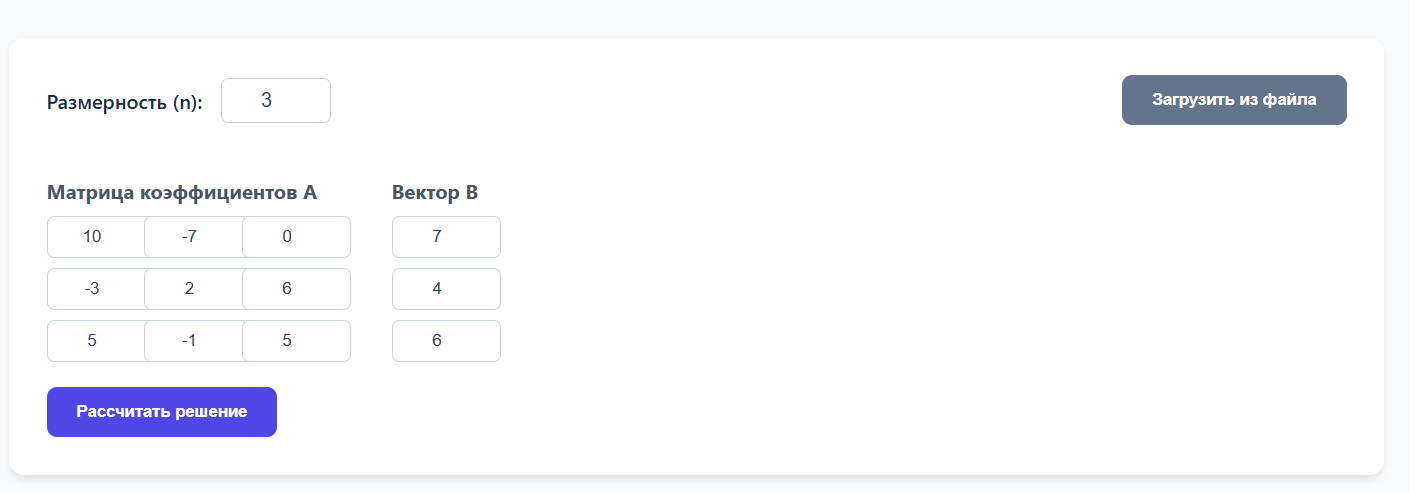
\includegraphics[width=0.9\textwidth]{screen_n3_input.png}
    \caption{Ввод данных для матрицы размерностью 3x3}
\end{figure}

\begin{figure}[H]
    \centering
    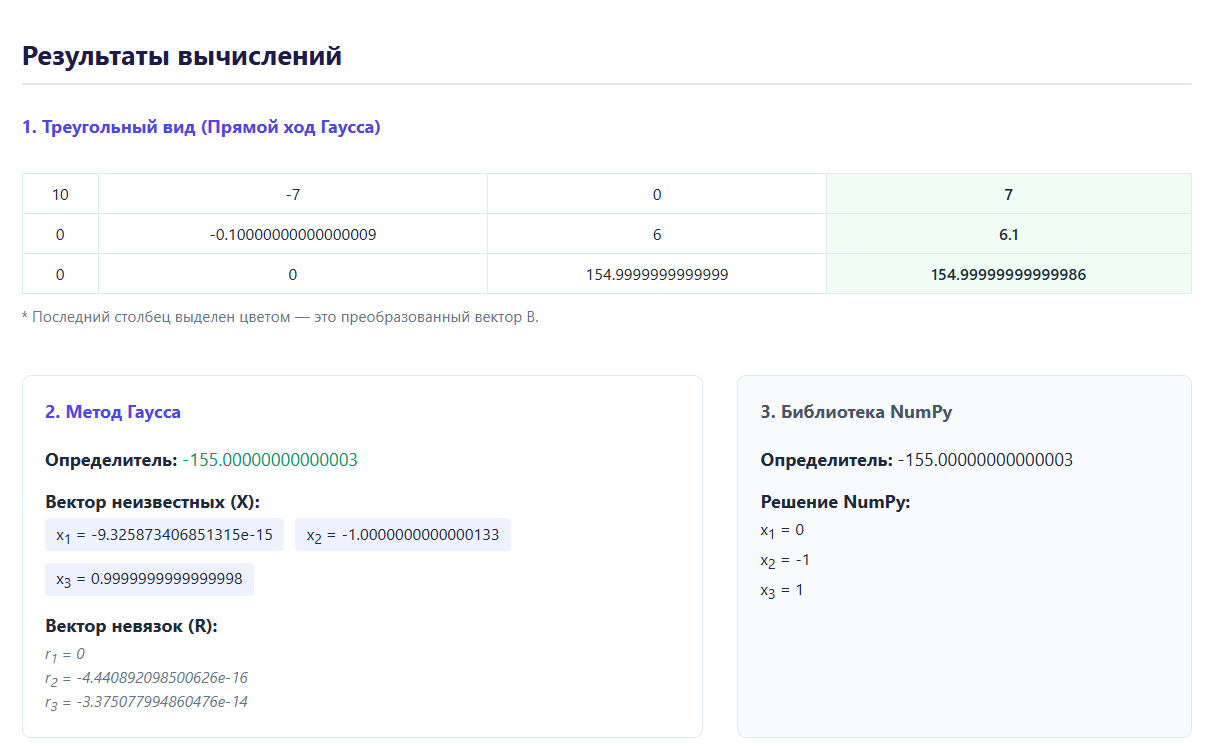
\includegraphics[width=0.9\textwidth]{screen_n3_output.png}
    \caption{Результаты вычислений для матрицы 3x3}
\end{figure}

\begin{figure}[H]
    \centering
    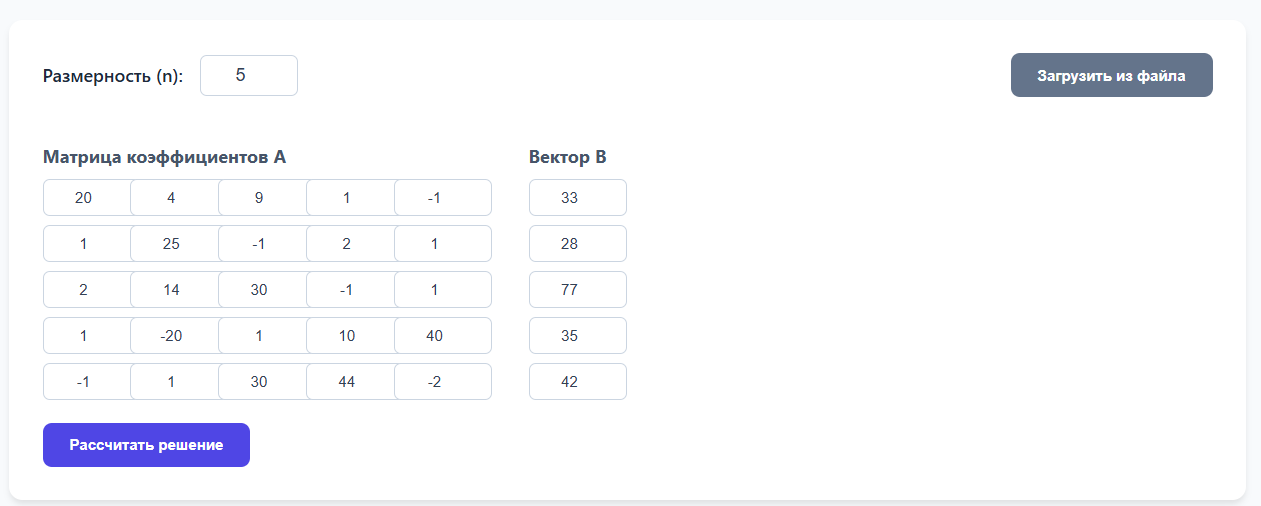
\includegraphics[width=0.9\textwidth]{screen_n5_input.png}
    \caption{Ввод данных для матрицы размерностью 5x5}
\end{figure}

\begin{figure}[H]
    \centering
    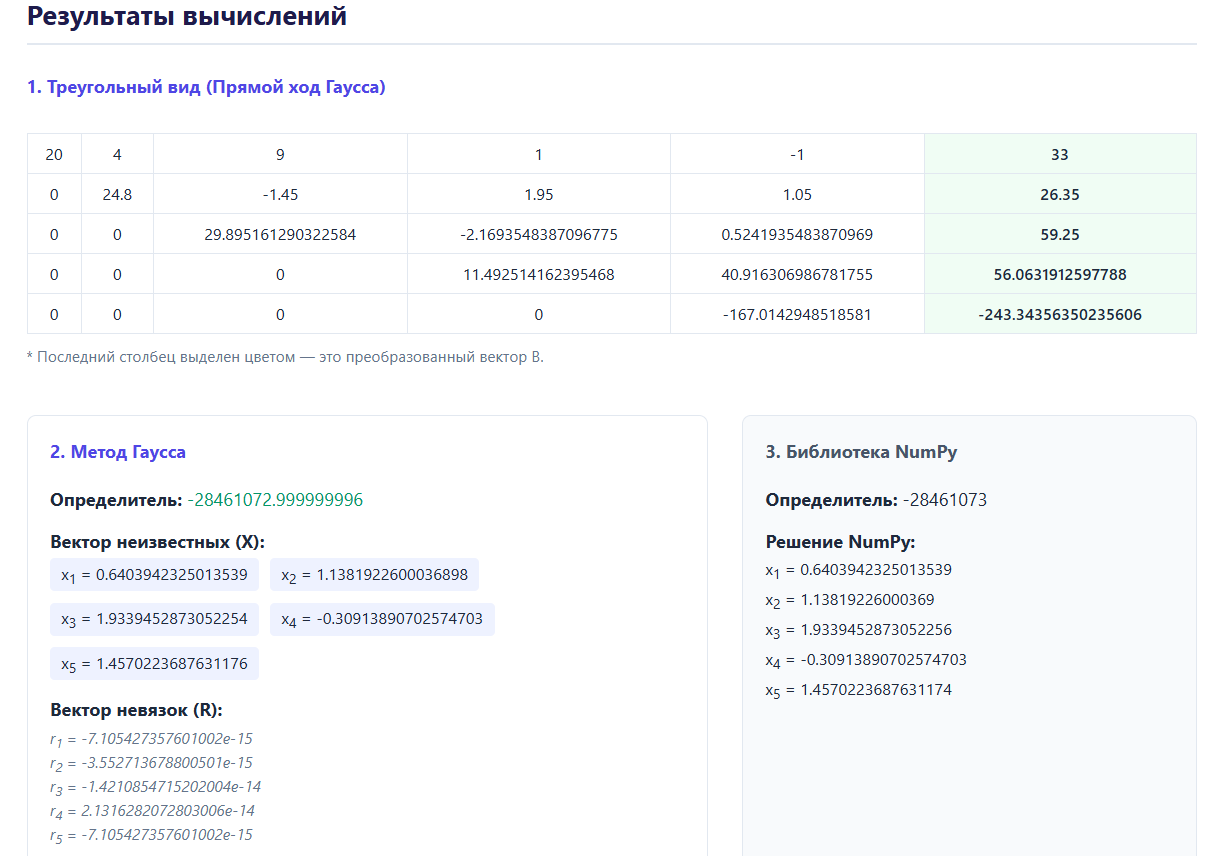
\includegraphics[width=0.9\textwidth]{screen_n5_output.png}
    \caption{Результаты вычислений для матрицы 5x5}
\end{figure}

\subsection*{Сравнение с эталонной библиотекой NumPy}

Анализ полученных результатов позволяет сделать вывод, что собственная реализация классического метода Гаусса успешно решает поставленную задачу. Вектор невязок для обеих тестовых систем близок к нулевому (компоненты вектора имеют порядок $10^{-14} \dots 10^{-16}$), что является отличным показателем точности. 

Однако при детальном сравнении результатов ручной реализации с ответами библиотеки \textbf{NumPy} наблюдаются характерные микроскопические различия, природа которых заключается в особенностях машинной арифметики:

\begin{enumerate}
    \item \textbf{Накапливаемая погрешность округления вещественных чисел:} \\
    В тесте размерности $n=3$ эталонная библиотека NumPy выдает точные целочисленные ответы: $x_1 = 0$, $x_2 = -1$, $x_3 = 1$. Наша реализация выдает значения: 
    $$x_1 = -9.325873406851315 \cdot 10^{-15}, \quad x_2 = -1.0000000000000133, \quad x_3 = 0.9999999999999998$$
    Это различие вызвано тем, что в классическом методе Гаусса многократно выполняются операции умножения, деления (особенно деление на ведущий элемент $a_{ii}$) и вычитания. Тип данных `float64` в стандарте IEEE 754 имеет ограниченную мантиссу (около 15-17 значащих десятичных цифр). С каждой новой операцией в младших разрядах накапливается погрешность. Библиотека NumPy внутри использует высокооптимизированные подпрограммы на C/Fortran (LAPACK/BLAS), которые могут применять более сложные стратегии выбора главного элемента или внутренне работать с повышенной точностью, а также аккуратнее форматировать финальный вывод.
    
    \item \textbf{Погрешность вычисления определителя:} \\
    Для матрицы $n=3$ определитель в обеих реализациях совпал с точностью до последних знаков ($-155.00000000000003$). Для матрицы $n=5$ реализованный метод выдал $\det \approx -28461072.999999996$, в то время как NumPy отобразил $-28461073$. В нашем алгоритме определитель считается как произведение диагональных элементов треугольной матрицы $\prod a_{ii}$. Поскольку сами диагональные элементы уже были получены в результате серии вычислений с плавающей точкой в ходе прямого хода, их погрешности перемножаются, давая небольшое отклонение от "идеального" математического значения на $16$-м знаке после запятой.
\end{enumerate}

Таким образом, выявленные различия между ответами NumPy и собственной реализацией не являются ошибками алгоритма. Они служат наглядной иллюстрацией накапливаемой вычислительной погрешности при работе с числами с плавающей точкой в прямых численных методах.

% ===========================================================================
% 7. Выводы
% ===========================================================================
\newpage
\section{Выводы}

В ходе выполнения лабораторной работы был изучен прямой метод решения систем линейных алгебраических уравнений — метод Гаусса. 

Был успешно реализован программный комплекс с клиент-серверной архитектурой (React + FastAPI), обеспечивающий:
\begin{itemize}
    \item Ввод данных как через динамическую веб-форму, так и путем загрузки файлов конфигурации.
    \item Прямой ход метода Гаусса для приведения матрицы к верхнетреугольному виду.
    \item Вычисление определителя системы на основе диагональных элементов треугольной матрицы.
    \item Обратный ход для вычисления искомого вектора неизвестных.
    \item Вычисление вектора невязок для оценки точности полученного решения.
\end{itemize}

Реализованная программа показала свою работоспособность на матрицах размерности $n \le 20$. Сравнение результатов самописного алгоритма с эталонным решением из библиотеки `NumPy` подтвердило корректность логики. Выявленные в ходе сравнения расхождения в младших разрядах дробной части (на уровне $10^{-15}$) успешно объяснены спецификой стандарта IEEE 754 и накоплением погрешности округления при делении и умножении вещественных чисел, что является нормальным поведением для численных методов. Вычисленный вектор невязок практически равен нулевому вектору, что свидетельствует о высокой точности найденного решения.

\end{document}